\begin{frame}[fragile]{GNU Radio Installation (4/7)}
\vspace{-1.0cm}
\footnotesize

\begin{itemize}
    \item \textbf{Verify the Python Installation.}

    \begin{itemize}
        \item \textbf{GNU Radio}
    \end{itemize}
\end{itemize}

\scriptsize
\begin{Verbatim}[xleftmargin=4.5em,breaklines,breaksymbolleft={},breaksymbolright={}]
python3 -c "from gnuradio import gr; print(gr.version())"
gnuradio_config_info --print-all
\end{Verbatim}

\footnotesize
\begin{itemize}
    \begin{itemize}
        \item \textbf{UHD}
    \end{itemize}
\end{itemize}

\scriptsize
\begin{Verbatim}[xleftmargin=4.5em,breaklines,breaksymbolleft={},breaksymbolright={}]
python3 -c "import uhd; print(uhd.get_version_string())"
\end{Verbatim}

\vspace{0.3cm}

\begin{center}
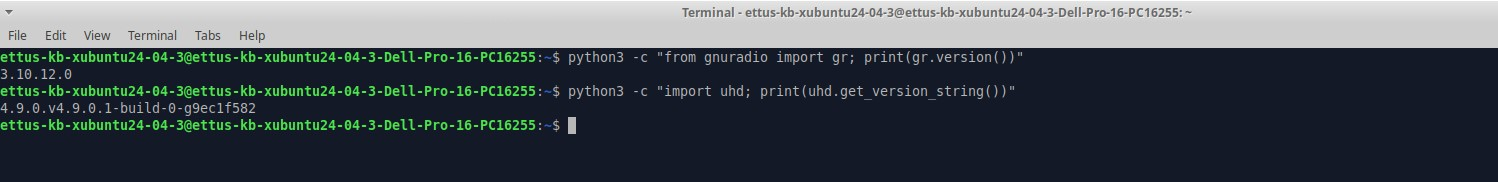
\includegraphics[width=0.8\linewidth]{latex/jpg_png/image_python verification GNU radio.jpg}
\end{center}

\end{frame}
